\section{결과와 연구 범위}

이번 PHYS18은 PHYS17에서 열린 HH--birth 혼합 응답을 실제로 계산한다.
PHYS16은 동일한 COMMON에서 시작한 두 half의 끝점 $g_2$와 Full의 끝점
$g_F$ 사이의 결함 $d=g_2-g_F$를 포함했고, PHYS17은
$d_\lambda,d_b$와 $F_\lambda<0$, $F_b>0$를 포함했다.
현재 질문은 birth를 바꿀 때 HH 방향의 온도 결함 응답이 얼마나 달라지는지,
또는 HH를 바꿀 때 birth 방향의 응답이 얼마나 달라지는지다.
두 질문의 공통 판별량은 $F_{\lambda b}$다.

\subsection{고정한 물리계와 입력}

매개변수는 동일한 전역 $\lambda,b\in[0,1]$이고, admissible $\alpha$를
고정한 원 source-aligned geometric-isotropic $C^2$ 계열을 사용한다.
기체 상태는 $g=(x_{\rm HII},y_{\rm HeII},y_{\rm HeIII},w)$이며
$w$의 단위는 ${\rm eV/H}$다. 광자 33개 군과 number/energy guard 두
좌표를 합친 35개 광자 좌표를 같은 연산 그래프에 유지한다.
두 half의 길이는 각각 $h=625000000\ {\rm s}$이고 Full의 길이는 $2h$다.
시각은 $t_0=160000000000$, $t_1=160625000000$,
$t_2=161250000000\ {\rm s}$다.

원 $C,B,q,S$는 PHYS15에 보존된 Full 자료다.
$q=\operatorname{exact64}(0.00011736830563768177)<1$과
$S=\operatorname{exact64}(0.015,0.01,0.01,0.5)$를 그대로 사용한다.
여기서 \texttt{exact64}는 저장된 binary64 leaf의 정확한 유리수 값이다.
온도 상수는 $C_T=2\,\mathrm{eV}_{\rm erg}/(3k_B)$이고,
$f_2=\operatorname{exact}(n_{\rm He,stored})/\operatorname{exact}(n_H)$,
$\ell_e=(1,f_2,2f_2,0)$를 사용한다.
$\Pi_2=1+f_2+\ell_e g_2$, $\Pi_F=\Pi_2-\ell_e d>0$에서 유한 분수를
계산한다. 원 $C^2$ 구간, root hull, 전처리 역 포함의 전제를 재사용한다.
상속 계약의 입력 24개는 크기와 SHA-256이 모두 일치했다.

\subsection{실제 혼합 포함}

혼합 도함수 $W=\partial_{\lambda b}g_2$와
$W_d=\partial_{\lambda b}(g_2-g_F)$는 보통의 편미분이며 Taylor 계수로
나누지 않는다. 표~\ref{tab:mixed-gas}는 최종 교차 포함을 보인다.

\begin{table}[H]
\centering\small
\caption{최종 mixed gas defect 포함. 두 매개변수는 무차원이다.}
\label{tab:mixed-gas}
\begin{tabular}{lll}\toprule
좌표 & 구간 & 단위 \\\midrule
$W_{d,x_{\rm HII}}$ & $[3.428209698898\times10^{-17},\ 4.498894132315\times10^{-17}]$ & 1 \\
$W_{d,y_{\rm HeII}}$ & $[-2.296697834724\times10^{-22},\ 5.758083648551\times10^{-23}]$ & 1 \\
$W_{d,y_{\rm HeIII}}$ & $[-9.420366340430\times10^{-24},\ -2.612148448548\times10^{-24}]$ & 1 \\
$W_{d,w}$ & $[-4.336773175632\times10^{-16},\ -3.600882004347\times10^{-16}]$ & $\mathrm{eV/H}$ \\
\bottomrule\end{tabular}
\end{table}


같은 양의 분모와 Full 온도 covector로 전달하면
\begin{equation}
 F_{\lambda b}\in[L_M,U_M]
 =[-2.668505746423,-2.118796636045]\times10^{-12}\ {\rm K}.
 \label{eq:main-mixed}
\end{equation}
이 수치는 exact rational endpoint를 바깥쪽으로 반올림한 표시다.
보존된 기계 결과에는 전체 유리수 양 끝점이 들어 있다.
따라서 $F_{\lambda b}<0$의 margin은 적어도 $2.118796636045\times10^{-12}\ {\rm K}$다.
입력 계열의 전체 사각형을 포함하는 판정이며 표본점 차분을 사용하지 않는다.

\begin{figure}[H]
\centering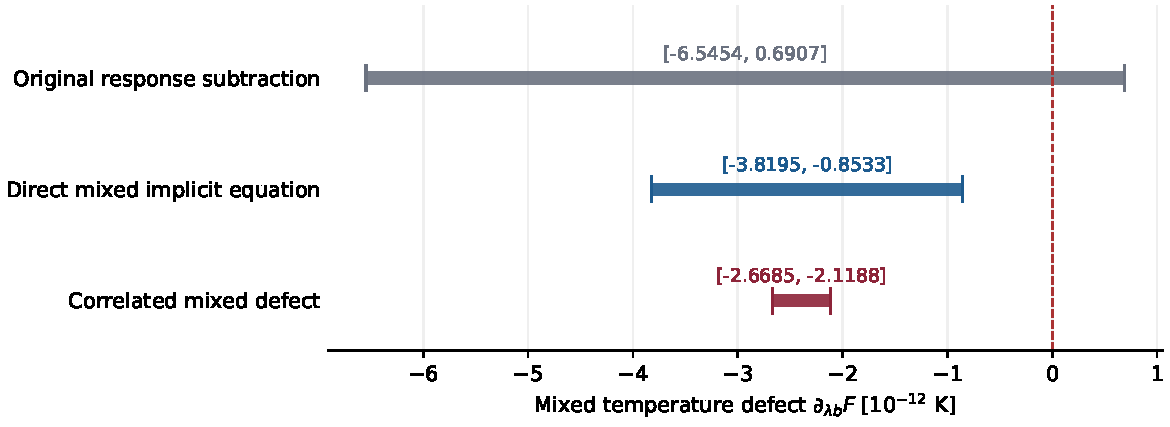
\includegraphics[width=0.97\linewidth]{figures/mixed_enclosure_comparison.pdf}
\caption{같은 유한 온도 분수에 전달한 세 가지 혼합 포함. 원 $W_2-W_F$
성분별 차는 0을 포함한다. 직접 암묵식은 음수를 판별하며, 작은 결함을
보존한 상관식은 가장 좁은 구간을 준다. 가로축은 $10^{-12}\ {\rm K}$다.}
\label{fig:comparison}
\end{figure}

\subsection{유한 매개변수 변화의 귀결}

$\lambda_1>\lambda_0$, $b_1>b_0$인 사각형에서 미적분학의 기본정리를
두 번 적용하면
\begin{align}
&F(\lambda_1,b_1)-F(\lambda_1,b_0)
-F(\lambda_0,b_1)+F(\lambda_0,b_0)\notag\\
&\qquad\in[L_M,U_M](\lambda_1-\lambda_0)(b_1-b_0)<0.
\label{eq:rectangle}
\end{align}
특히 단위 사각형의 $\mathcal I$도 식~\eqref{eq:main-mixed}의 구간에 들어간다.
이전 PHYS17의 $|\mathcal I|\le1.958485175177039\times10^{-9}\ {\rm K}$에
비해 현재 절댓값 상계는 약 734배 작고 부호도 결정된다.

$b$가 커지면 $F_\lambda$는 더 음수가 되고, $\lambda$가 커지면
양수인 $F_b$는 조금 줄어든다. 두 1차 방향의 부호는 PHYS17의 전역
구간에 의해 유지된다. 혼합 변화의 크기는 HH 1차 방향의 최소 절댓값에
대해 약 $0.033\%$ 이하, birth 1차 방향에 대해 약
$3.94\times10^{-6}\%$ 이하다.

축 위의 정확한 응답으로 만든 가법 표현
$F_{\rm sep}(\lambda,b)=F(\lambda,0)+F(0,b)-F(0,0)$에 대해서는
\begin{equation}
F(\lambda,b)-F_{\rm sep}(\lambda,b)
\in[L_M,U_M]\lambda b.
\label{eq:separable}
\end{equation}
따라서 이 가법 표현은 내부에서 실제 $F$보다 크며, 그 오차는 최대
$2.668506\times10^{-12}\lambda b\ {\rm K}$로 포함된다.
축 위 응답 자체를 새로 근사할 때의 오차는 그 근사 계약에 따로 포함한다.

\subsection{물리적 구성과 폭의 원인}

고정된 기체에서 원 $H_{\lambda b}=0$이다. 실제 혼합 응답은 기체의
암묵적 변화, 광자 흡수의 상태 의존성, 유한 온도의 입자수 분모에서 생긴다.
같은 $J_F^{-1}$와 같은 온도 covector로 각 강제항을 전달하여 이 연결을
분리했다. 가장 큰 음의 항 두 개는 HH 기울기를 stage birth 변화와
endpoint birth 결함에 각각 작용시킨 항이다. birth의 backward Euler
혼합 항, 흡수율 변화, 온도 분모 항도 음의 방향으로 더해진다.

\begin{table}[H]
\centering\small
\caption{Full 역연산자로 전달한 강제항 묶음과 유한 온도 분모의 별도 기여. 단위 K.}
\label{tab:groups}
\begin{tabular}{ll}\toprule
묶음 & 온도 혼합 기여 \\\midrule
HH 기울기 묶음 & $[-2.329668009361\times10^{-12},\ -1.928397581837\times10^{-12}]$ \\
일곱 광자 항 & $[-3.024678223968\times10^{-13},\ -1.735793802686\times10^{-13}]$ \\
나머지 기체와 endpoint 항 & $[2.819648272515\times10^{-16},\ 1.140914739344\times10^{-15}]$ \\
온도 분모와 기하 항 & $[-3.666218766444\times10^{-14},\ -1.794167181955\times10^{-14}]$ \\
\bottomrule\end{tabular}
\end{table}


\clearpage
